\chapter{Path planning theory}
An autonomous system must be able to create a plan on how the system should move around in the surrounding environment in a feasible way. A minimum requirement for a path is that it is connected. The connection level can be described by the paths smoothness. Geometric continuity is a relaxed from of parametric continuity in witch discontinuousness in speed is allowed. Geometric continuity is sufficient for a path following system, witch is the main focus of this thesis. Geometric continuity is denoted as $G^n$ were n is the order of continuity.

Smoothness level in this thesis is follow the the definition given by Anastasios M. Lekkas Lecture 1.

\begin{table}[H]
\begin{center}
\begin{tabular}{| l | | l |}
\hline
\textbf{Geometrical smoothness level} & \textbf{Description} \\ \hline
$G^0$ & All subpaths are connected \\ \hline
$G^1$ & The path-tangential angle is continuous \\ \hline
$G^2$ & The center of curvature is continuous \\ \hline
\textbf{Parametric smoothness level} & \textbf{Description} \\ \hline
$C^0$ & All subpaths are connected \\ \hline
$C^1$ & The velocity is continuous \\ \hline
$C^2$ & The acceleration is continuous \\ \hline
\end{tabular}
\end{center}
\caption{Smoothness definitions}
\label{TB:SmoothnessDescriptions}
\end{table} 

A the definition that is used for path in this thesis is:
\begin{equation}
P_s(x_s,y_s,z_s,\psi_s) \rightarrow P_f(x_f,y_f,z_f,\psi_f)
\end{equation}
were the subscripts $s$ and $f$ denaontes the start pose and finish pose respectfully. This is an relaxed form of the start and finish pose since the pitch and roll angle is assumed stable, and therefore a desired start and finish value is not required.

\section{Straight lines}
The simplest form on path is a straight line between $P_s$ and $p_f$. The straight line is given as 
\begin{subequations}
\begin{align}
& x(t) = a_xt + b_x \\
& y(t) = a_yt + b_y 
\end{align}
\end{subequations}
with $ t \in [0,1] $. Then the parametrisation of the straight line is:
\begin{subequations}
\begin{align}
& x(0) = b_x \rightarrow b_x = x_s \\
& x(1) = x_f = a_x + b_x \rightarrow a_x = x_f - b_x \\
& y(0) = b_y \rightarrow b_y = y_s \\
& y(1) = y_f = a_y + b_y \rightarrow a_y = y_f - b_y \\
\end{align}
\end{subequations}
A path constructed by straight lines is $G^0$ and $C^0$, however since the tangential vector is discontinuous between two line segments with different heading it's not $G^1$ or $C^1$.
The simplest for of creating a path is a straight line between two way-points. The advantage with a straight line is that it's easy for a guidance system to follow the line, however it will experience a jump in reference when transitioning to another straight line due to discontinuous tangential vector.
\section{Dubins path}\label{S:DubinsPath}
An alternative to a straight line path is a path constructed by straight lines and circle. Rudolf Dubin showed \citep{dubins1957curves} that the shortest possible path for a particle that moved with unit speed with maximum curvature would consist of three pieces. The path is considered as the shortest path from $P_s$ to $P_f$, however the curvature is discontinues, which gives a smoothness level of $G^1$ and $C^0$. 
Dubins path is the shortest path from from one way-point to the other which is continues. Dubins path can be created for a three dimensional case, however a simplification is made in which only a planar version of the Dubins path is examined. A Dubin path with fixed end orientation can be constructed in four different way.
\begin{table}[H]
\centering
\begin{adjustbox}{max width=\textwidth}
\begin{tabular}{ | l |}
\hline
Right to Right \\
Right to left \\
Left to Right \\
Left to left \\ \hline
\end{tabular}
\end{adjustbox}
\end{table}

Allowing the finish orientation to be free will add four more variants of the Dubins path.
The path consist of two arcs and a straight line. The straight line is tangential to both arcs. The start and end point of the straight line can be found with
\begin{subequations}
\begin{align}
& \alpha = \arcsin\big(\frac{\rho_f-\rho_s}{|c|}\big) \\
& \beta = \arctan\big(\frac{y_{cf}-y_{cs}}{x_{cf}-x_{cs}}\big)
\end{align}
\end{subequations}

\begin{table}[H]
\begin{center}
\begin{tabular}{ | l | | l |}
\hline
& \textbf{Turn angle} \\ \hline
$\phi_{right}$ & $\alpha + \beta + \frac{\pi}{2}$ \\
$\phi_{left}$ & $\beta - \alpha + \frac{3\pi}{2}$ \\ \hline
\end{tabular}
\end{center}
\end{table}

\begin{subequations}
\begin{align}
& x_{P_\chi} = x_{cs} + R_s\cos(\phi) \\
& y_{P_\chi} = x_{cs} + R_s\sin(\phi) \\
& x_{P_N} = x_{cf} + R_f\cos(\phi) \\
& y_{P_N} = x_{cf} + R_f\sin(\phi)
\end{align}
\end{subequations}
\begin{figure}[H]
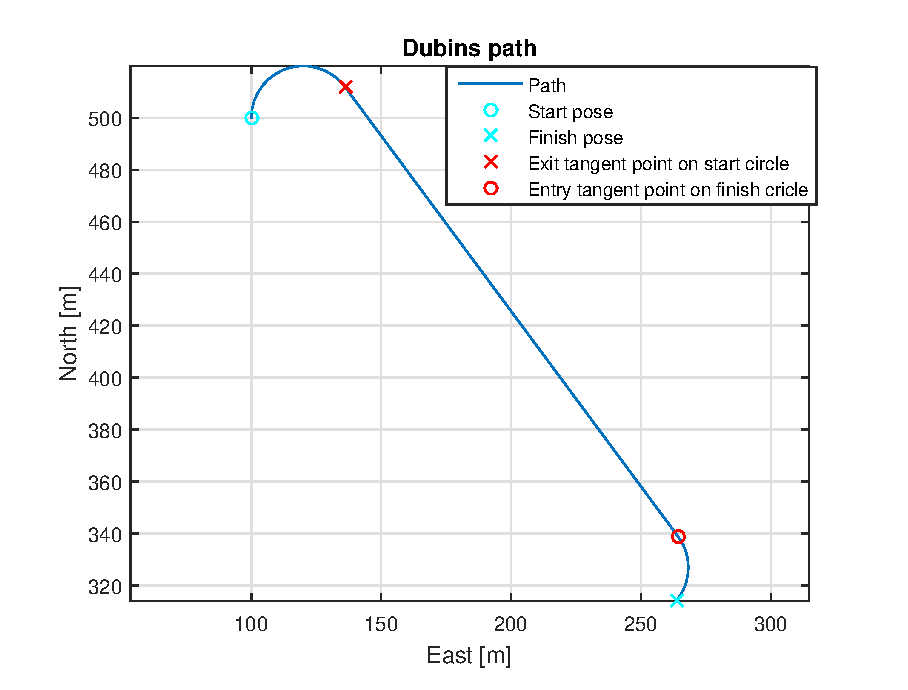
\includegraphics[width=0.7\textwidth]{figs/TheoryPlot/DubinsPath.eps}
\end{figure}